\begin{anexosenv}
% \partanexos

\chapter{BATERIA}

Este anexo apresenta uma imagem ilustrativa da bateria selecionada para o projeto.

\begin{figure}[H]
    \centering
    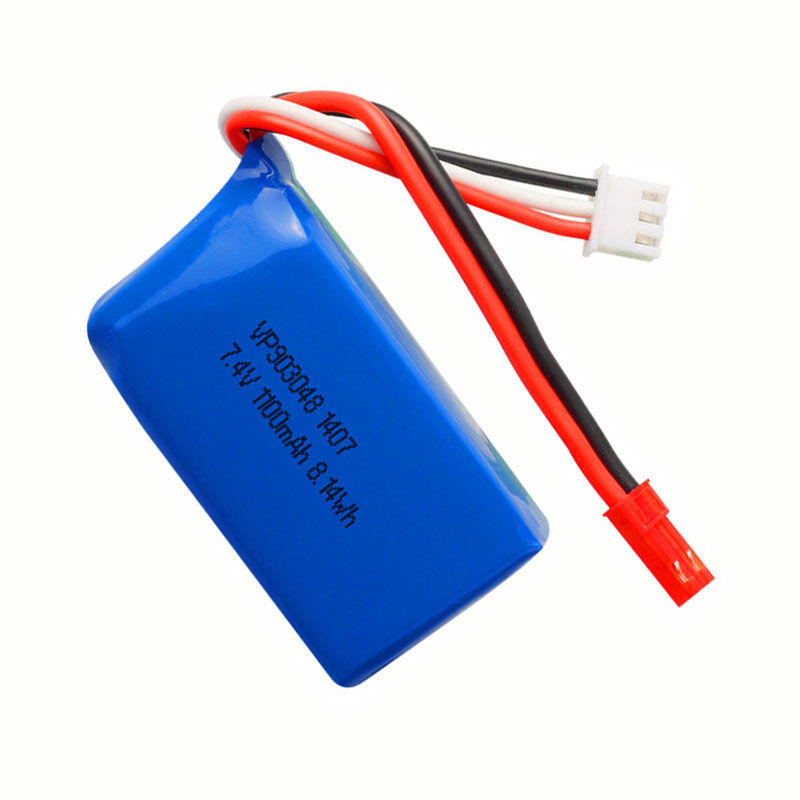
\includegraphics[width=0.6\textwidth]{figuras/imagembateria.png}
    \captionsetup{font=footnotesize}
    \caption{Imagem ilustrativa da bateria selecionada.}
\end{figure}

% \textcolor{red}{Apêndices e anexos são materiais complementares ao texto que só devem ser incluídos quando forem imprescindíveis à compreensão deste:}

% \textcolor{red}{
% \begin{itemize}
%     \item Apêndices são textos elaborados pelo autor a fim de complementar sua argumentação.
%     \item Anexos são os documentos não elaborados pelo autor, que servem de fundamentação, comprovação ou ilustração, como mapas, leis, estatutos etc.
% \end{itemize}}
% \textcolor{red}{\textbf{Texto do primeiro anexo.}}

% \chapter{Segundo Anexo}
% \textcolor{red}{Apêndices e anexos são materiais complementares ao texto que só devem ser incluídos quando forem imprescindíveis à compreensão deste:}

% \textcolor{red}{
% \begin{itemize}
%     \item Apêndices são textos elaborados pelo autor a fim de complementar sua argumentação.
%     \item Anexos são os documentos não elaborados pelo autor, que servem de fundamentação, comprovação ou ilustração, como mapas, leis, estatutos etc.
% \end{itemize}}
% \textcolor{red}{\textbf{Texto do segundo anexo.}}

% \begin{figure}[htpb]
% \centering
% 
\includegraphics[width=\textwidth]{figuras/fga.png}
% \caption{Figura do Anexo 2.}
% \label{fig:fig_anexo}
% \end{figure}

\end{anexosenv}
